\documentclass[11pt,a4paper]{article}
\usepackage{{../../paquete-formulas}}
\usepackage{{../../estilos-formulas}}
\usepackage{enumitem}
\usepackage{multirow}
\usepackage[document]{ragged2e}

\newcommand{\materia}{Elementos de Máquinas}

\begin{document}
\pagestyle{pieyencabezado}
% \setlength\itemsep{-3mm}

\begin{multicols}{2}	
	\begin{cajita}
		\section*{5 teorías de rotura}
		\begin{flushleft}
			1- Máxima tensión corte (GUEST):
			\begin{equation*}
				\dfrac{\sigma_{T}}{C_{s}}=\sigma_{adm}\geq\sqrt{(\sigma_{x}-\sigma_{y})^{2}+4~\tau_{xy}^{2}}
			\end{equation*}
			2- Máxima tensión normal:
			\begin{equation*}
				\dfrac{\sigma_{RT}}{C_{s}}=\sigma_{adm}\geq\dfrac{\sigma_{x}+\sigma_{y}}{2}+\dfrac{1}{2}\sqrt{(\sigma_{x}-\sigma_{y})^{2}+4~\tau_{xy}^{2}}
			\end{equation*}
			3- Deformaciones principales:
			\begin{equation*}
				\dfrac{\sigma_{RT}}{C_{s}};\dfrac{\sigma_{RC}}{C_{s}}=\sigma_{adm}
			\end{equation*}
			\begin{equation*}
				\sigma_{adm}\geq(\sigma_{x}-\sigma_{y})\left(\dfrac{1-\mu}{2}\right)\pm\dfrac{1+\mu}{2}\sqrt{(\sigma_{x}-\sigma_{y})^{2}+4~\tau_{xy}^{2}}
			\end{equation*}
			4- Energía deformación
			\begin{equation*}
				\sigma_{adm}=\dfrac{\sigma_{f}}{Cs}\geq\sqrt{\sigma_{x}^{2}+\sigma_{y}^{2}-2\mu \sigma_{x} \sigma_{y} +2(1+\mu)\tau_{xy}^{2}}
			\end{equation*}
			5- Energía distorión:
			\begin{equation*}
				\sigma_{adm}=\dfrac{\sigma_{f}}{Cs}\geq\sqrt{\sigma_{x}^{2}-\sigma_{x} \sigma_{y}+\sigma_{y}^{2}+3\tau_{xy}^{2}}			
			\end{equation*}
		\end{flushleft}
			\begin{tabular}{l r}
				(1,4,5 $\rightarrow$ material dúctil) & (2,3 $\rightarrow$ material frágil)
			\end{tabular}
		

	\begin{cajita}
%		\vspace{0.5cm}
		\textbf{NOMENCLATURA}
		\begin{tabular}{l r}
			$\sigma_{T}$&tensión tracción \\
			$\sigma_{C}$&tensión compresión\\
			$\sigma_{f}$&tensión fluencia\\
			$\sigma_{adm}$&tensión admisible\\
			$Cs$&Coeficiente de seguridad\\
		\end{tabular}
	\end{cajita}
	\end{cajita}

	\begin{cajita}
		\section*{Deformaciones}
		\begin{center}
			$e=\dfrac{l-l_{0}}{l_{0}}$
		\end{center}
		\begin{itemize}[itemsep=-2mm]
			\item $e$ = alargamiento especifico.
			\item $l$ = longitud "final"
			\item $l_{0}$ = longitud inicial
		\end{itemize}
	
		\begin{center}
			$\sigma=E~e$
		\end{center}
%		\begin{itemize}[itemsep=-2mm]
%			\item $e$ = alargamiento especifico.
%			\item $l$ = longitud "final"
%			\item $l_{0}$ = longitud inicial
%		\end{itemize}
	\textbf{	Para deformaciones producidas por torsión}
	\begin{center}
		$\tau_{xy}=G~ \gamma$\hspace*{1.5cm}$G=\dfrac{E}{2(1+\mu)}$
	\end{center}
	\begin{itemize}[itemsep=-2mm]
		\item $\tau$ = tensión tangencial
		\item $\gamma$ = angulo distorsión
		\item $l_{0}$ = longitud inicial
	\end{itemize}
	\end{cajita}

	\begin{cajita}
	\section*{Cargas dinámicas}
	\textbf{Solicitud dinámica axial}\\
	\begin{center}
		$\delta=\delta_{est}\left(1+\sqrt{1+\dfrac{v^{2}}{g~\delta_{est}}}\right)$
	\end{center}
	\begin{itemize}[itemsep=-2mm]
		\item $\delta_{est}$ alargamiento estático
		\item $v$ velocidad
		\item $g$ gravedad
	\end{itemize}
	\begin{center}
	$\sigma_{din}=\sigma_{est}\left(1+\sqrt{1+\dfrac{2~h}{\delta_{est}}}\right)$
	\end{center}
	\begin{itemize}[itemsep=-2mm]
		\item $\sigma_{est/din}$ tensión estatica/dinamica
		\item $h$ altura
	\end{itemize}
	
	\end{cajita}


	\begin{cajita}
		\section*{Tensiones variables}
		\begin{cajita}
			\textbf{Consideraciónes/Recordatorios}\\\vspace{0.2cm}
%			$\tau_{f}=0.6~\sigma_{f}$ ||| $\tau_{max}=\dfrac{MT}{Wp}=\dfrac{MT~16}{Pi~D^{3}}$
			\begin{tabular}{l|r}
%				\multicolumn{2}{r}{Esto aplica para cilindros}\\
			\multirow[r]{2}{2.5 cm}{Esto aplica para cilindros}& $\tau_{max}=\dfrac{MT}{Wp}=\dfrac{MT~16}{\pi~D^{3}}$\\[0.3 cm]
				& $\sigma_{max}=\dfrac{MF}{Wr}=\dfrac{MF~32}{\pi D^{3}}$\\[0.2 cm]
			\end{tabular}\\\vspace{0.2cm}
		
		$\tau_{f}=0.6~\sigma_{f}$ y tambien $\tau_{R}=0.6~\sigma_{R}$ \\\vspace{0.3cm}
		
		$\mathbf{\sigma_{wb}}$ para distintos materiales\\\vspace*{0.2cm}
			\begin{tabular}{l|r}
				Aceros	& 0.4 / 0.5 $\sigma_{R}\leq140Kg/mm^{2}$\\
				\multicolumn{2}{r}{ 70 $kg/mm^{2}$ si$\sigma_{R}\geq140Kg/mm^{2}$}\\
				Fundición & 0.4 $\sigma_{R}$\\
				Al y Mg & 0.3 /0.4$\sigma_{R}$\\
				
			\end{tabular}
		
			
		
		\end{cajita}
		\begin{tabular}{l r}
			Tension media & tension alternada\\
			$\sigma_{m}=\dfrac{\sigma_{max}+\sigma_{min}}{2}$&$\sigma_{a}=\dfrac{\sigma_{max}-\sigma_{min}}{2}$\\[0.3cm]
			\multicolumn{2}{c}{$\sigma_{max}=\sigma_{m}+\sigma_{a}$}\\[0.3cm]
			Criterio Soderberg & $Cs=\dfrac{\sigma_{f}}{\sigma_{m}+\sigma_{a}*K_{f}*\dfrac{\sigma_{f}}{\sigma_{w}^{*}}}$\\[0.3cm]
			& $Cs=\dfrac{\tau_{f}}{\tau_{m}+\tau_{a}*K_{f}*\dfrac{\tau_{f}}{\tau_{w}^{*}}}$\\
		\end{tabular}\\
	\textbf{Factores de concentración}
	
	$K_{t}=\dfrac{\sigma_{máx}}{\sigma_{nominal}}$, sale de ábaco.\\ \vspace*{0.2cm}
	$K_{f}=1+q*\left(K_{t}-1\right)$
		\begin{itemize}[itemsep=-2mm]
		\item $q$ Indice de entalladura $\rightarrow$ Syrson
		\item $K_{t}$ factor geométrico
		\item $K_{f}$ factor geométrico,tamaño absoluto.
	\end{itemize}

	\textbf{Coef. seguridad}\\
		\begin{tabular}{l r}
			\hline
			Cond. Estática & Cond. Fatíga\\
			$Cs=\dfrac{\sigma_{f}}{\sigma_{máx}}=\dfrac{\sigma_{f}}{\sigma_{m}+\sigma_{a}}$ & $Cs=\dfrac{\sigma_{w}^{*}}{\sigma_{a}*K_{f}}$ \\
			\multicolumn{2}{r}{ $K_{f}$ solo si hay concentración} \\
			\hline
		\end{tabular}
	
%	\vspace*{0.4cm}
	\newpage
	
	\textbf{VIDA}\\
	\textbf{Finita}\\
	

	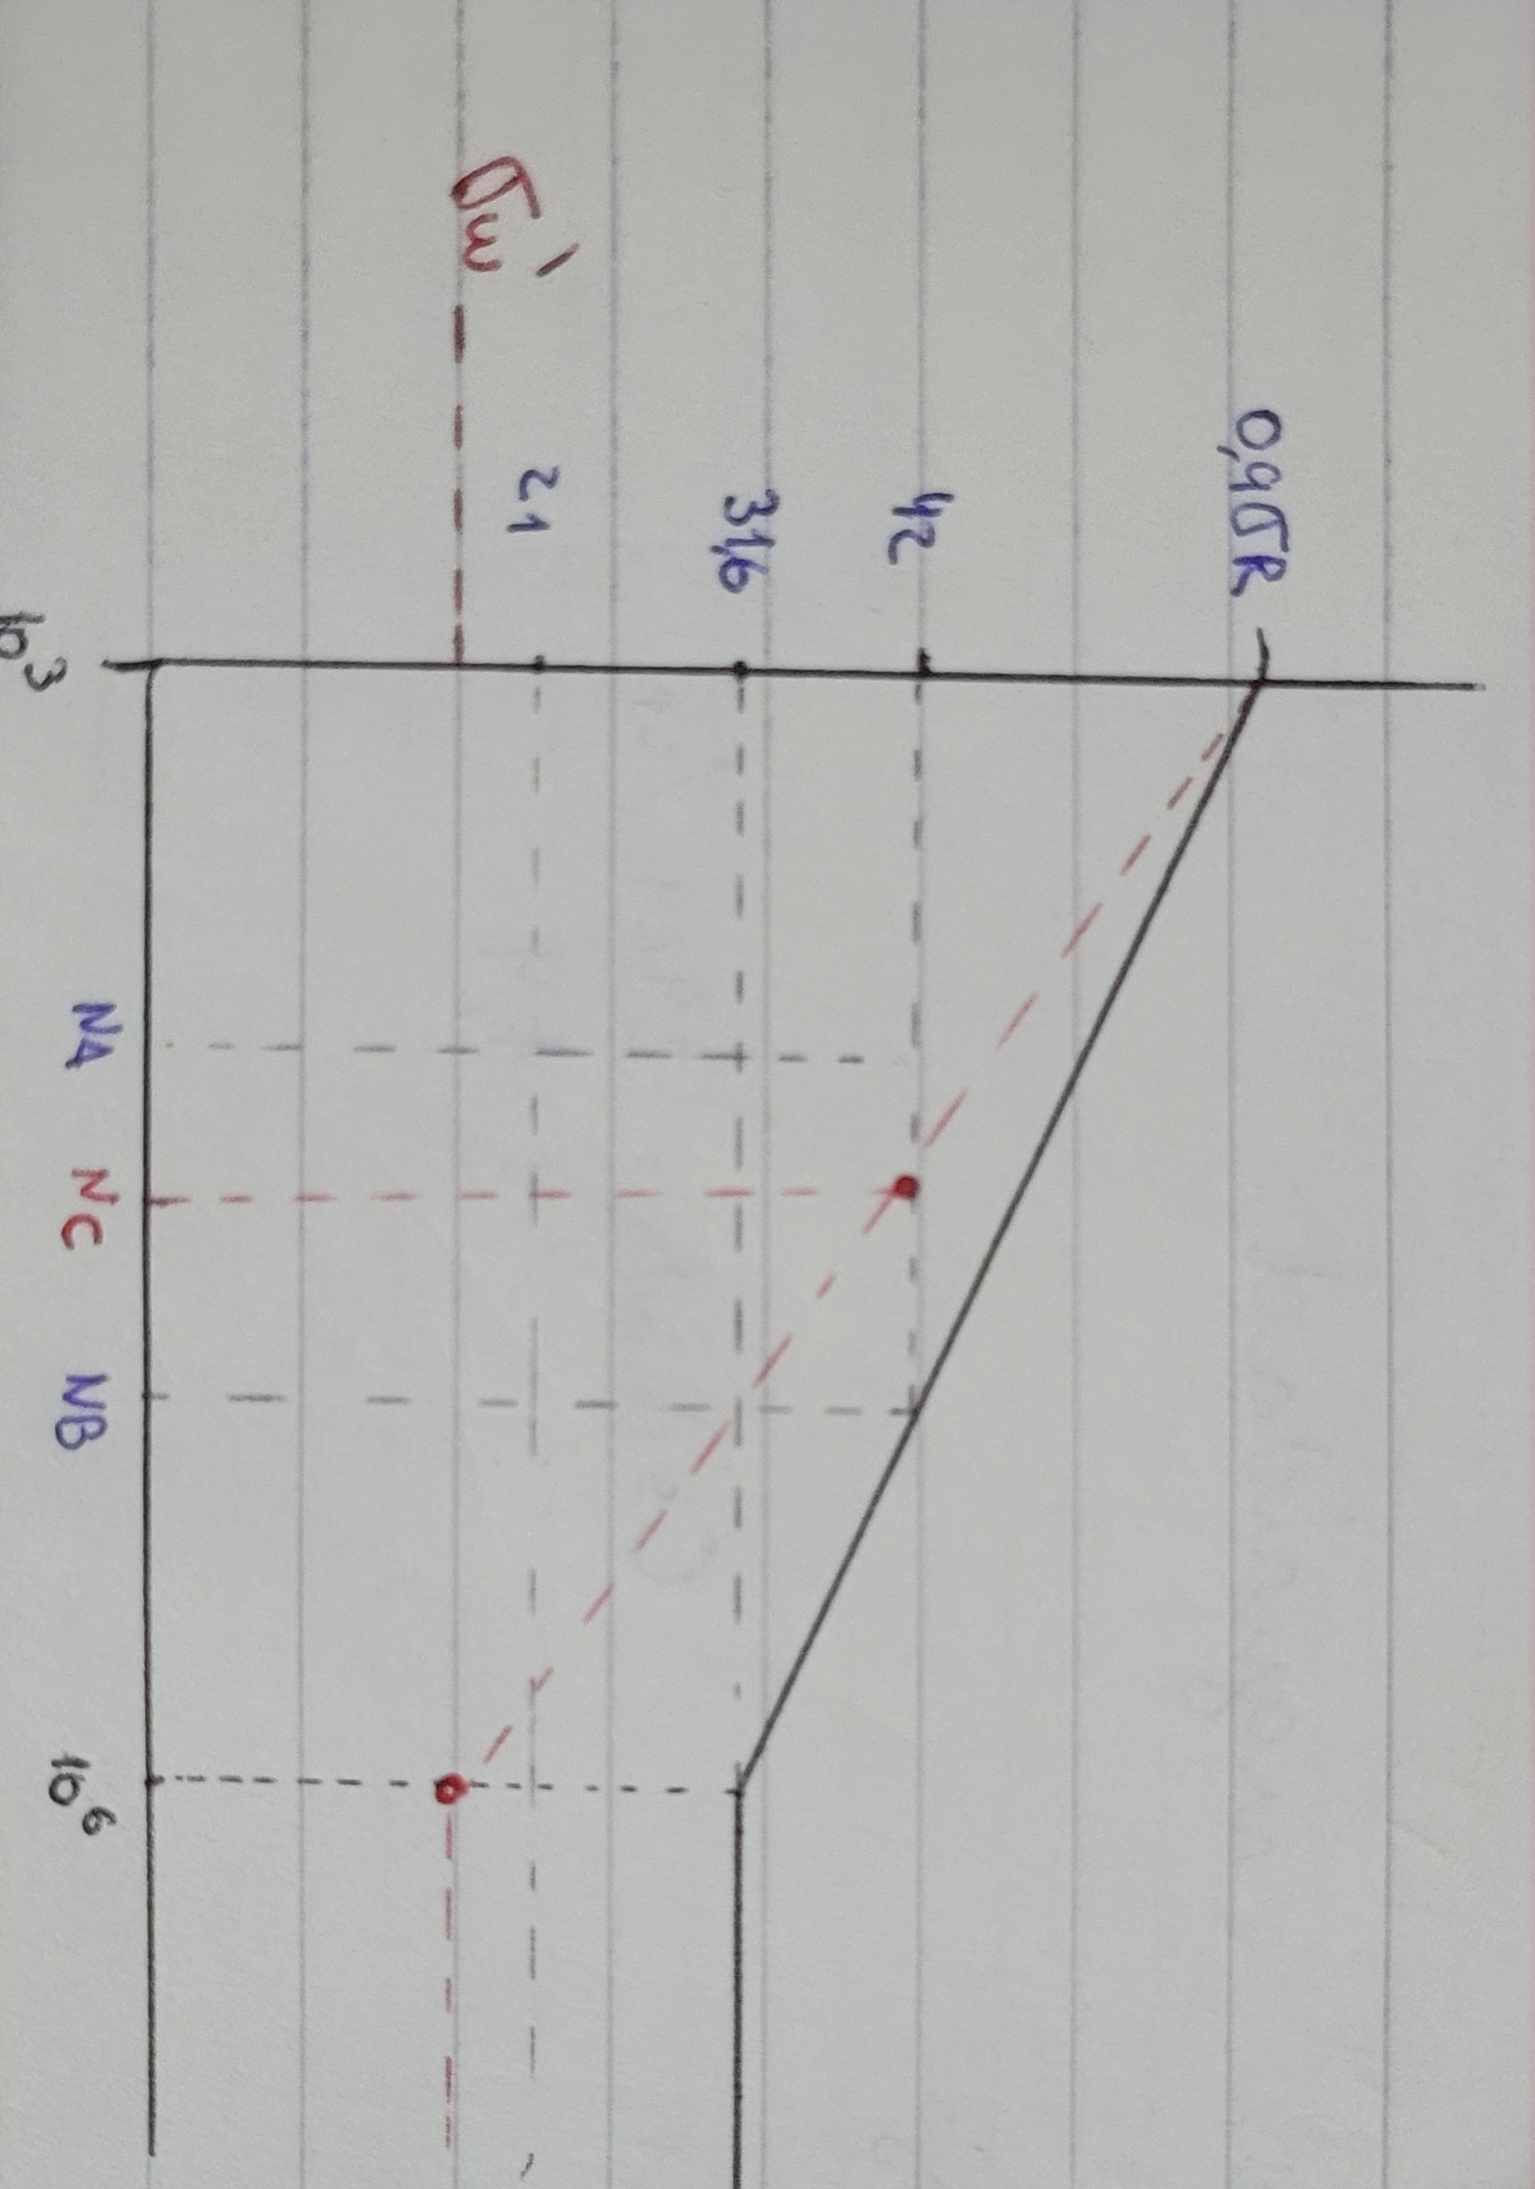
\includegraphics[height=0.8\textwidth, angle=90]{fluencia}
	
%		\begin{figure}
%%			\vspace{-1cm}
%			\centering
%			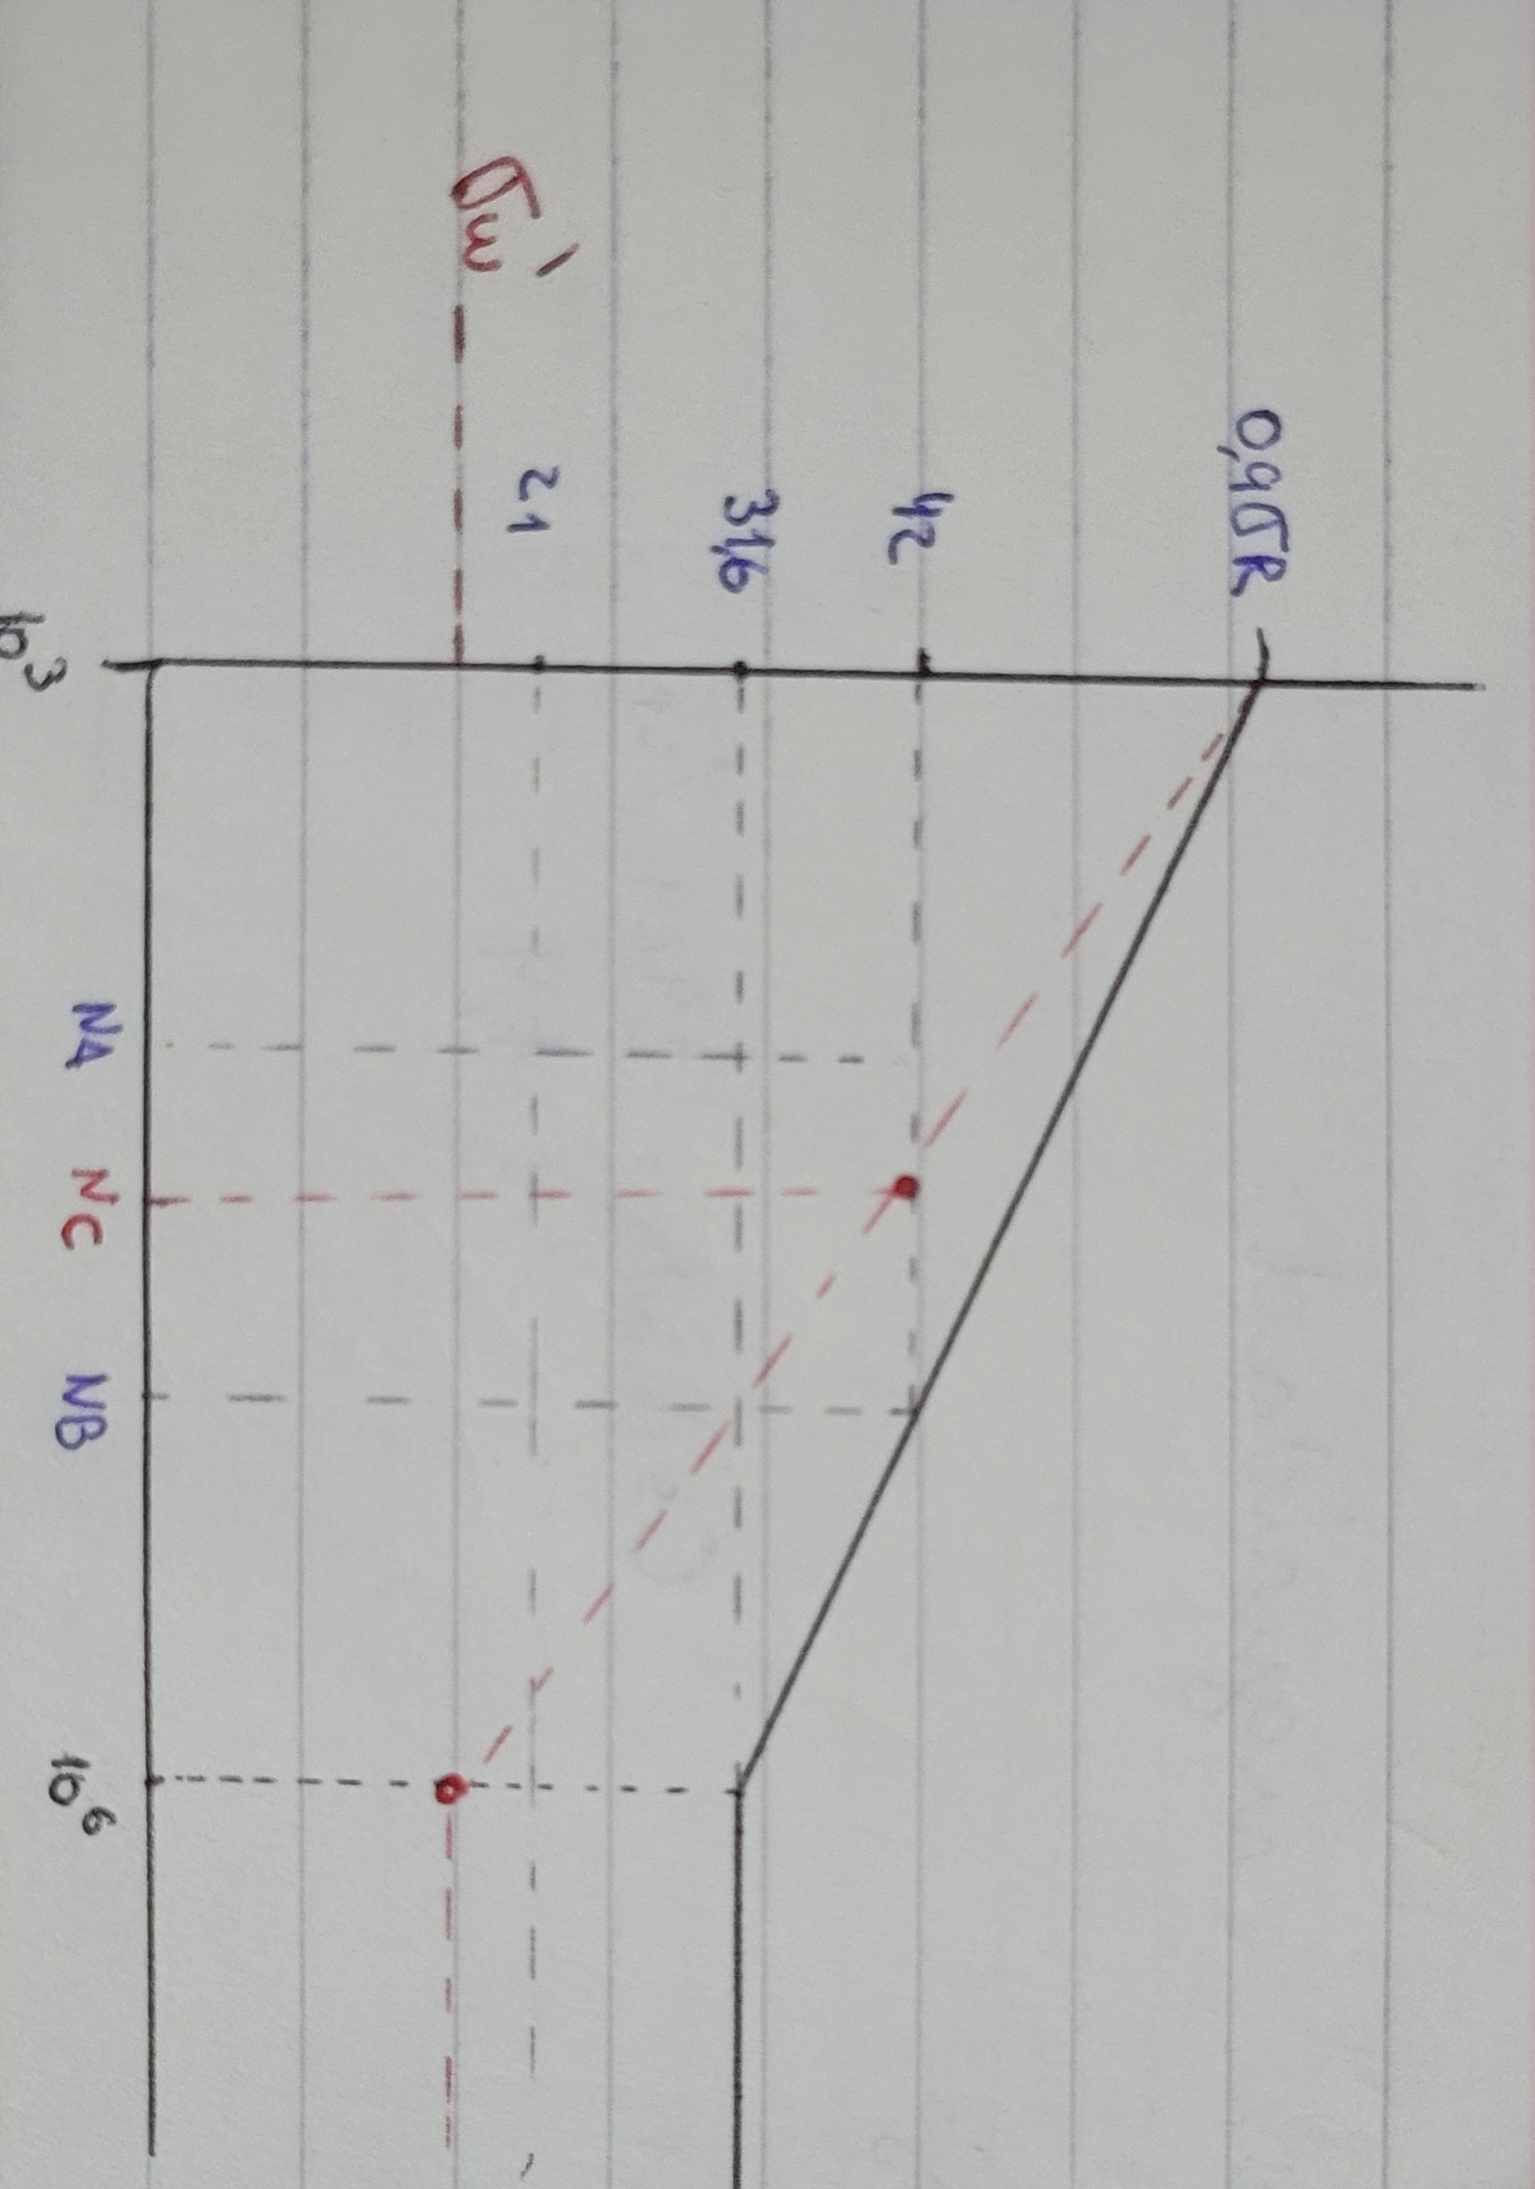
\includegraphics[height=0.8\textwidth, angle=90]{fluencia}
%		\end{figure} % YO NO ENTIENDO PORQUE ESTA VERGA NO ANDA
	
	
	
	
	\begin{tabular}{r l }
		\multicolumn{2}{c}{Condicionando cantidad de RPMs/ciclos}\\
		$m=\dfrac{1}{3}log_{10}\left(\dfrac{0.9\sigma_{R}}{\sigma_{w}}\right)$&
		$b=log_{10}\left(\dfrac{0.9\sigma_{R}^{2}}{\sigma_{w}}\right)$\\[0.5cm]
		$\sigma_{wN}=\left[\dfrac{10^{b}}{N_{(RPM)}^{m}}\right]$& $N_{(RPM)}=\sqrt[m]{\dfrac{10^{b}}{\sigma_{wN}}}$\\[0.5cm]
		\multicolumn{2}{c}{$CL=\dfrac{\sigma_{wN}}{\sigma_{w}}$}\\
	\end{tabular}

	\begin{tabular}{r l }
		\multicolumn{2}{c}{Vida restante en caso de sobrecarga}\\[0.2cm]
		$m=\dfrac{1}{3}log_{10}\left(\dfrac{0.9\sigma_{R}}{\sigma_{w}^{*}}\right)$&
		$b=log_{10}\left(\dfrac{0.9\sigma_{R}^{2}}{\sigma_{w}^{*}}\right)$\\[0.5cm]
		$Nb_{(RPM)}=\left[\dfrac{10^{b}}{\sigma_{N}}\right]^{\frac{1}{m}}$&$Nc~=~Nb~-~Na$\\
		la nueva tension: & $\sigma_{w}^{'}=\left[\dfrac{10^{b^{'}}}{N_{(RPM)}^{m^{'}}}\right]$\\[0.5cm]
		\multicolumn{2}{l}{$m^{'}=\dfrac{log_{10}(0.9\sigma_{R})-log_{10}(\sigma_{N})}{log_{10}Nc-log_{10}10^{3}}$}\\[0.3cm]
		\multicolumn{2}{l}{$b^{'}=log_{10}(0.9\sigma_{R})+m^{'}~(log_{10}10^{3})$}\\[0.25cm]
		
%		$\sigma_{wN}=\left[\dfrac{10^{b}}{N_{(RPM)}^{m}}\right]$& \\[0.5cm]
%		\multicolumn{2}{c}{$CL=\dfrac{\sigma_{wN}}{\sigma_{w}}$}\\
	\end{tabular}
\end{cajita}
\newpage
\begin{cajita}

	\textbf{Diagrama de Goodman}\\
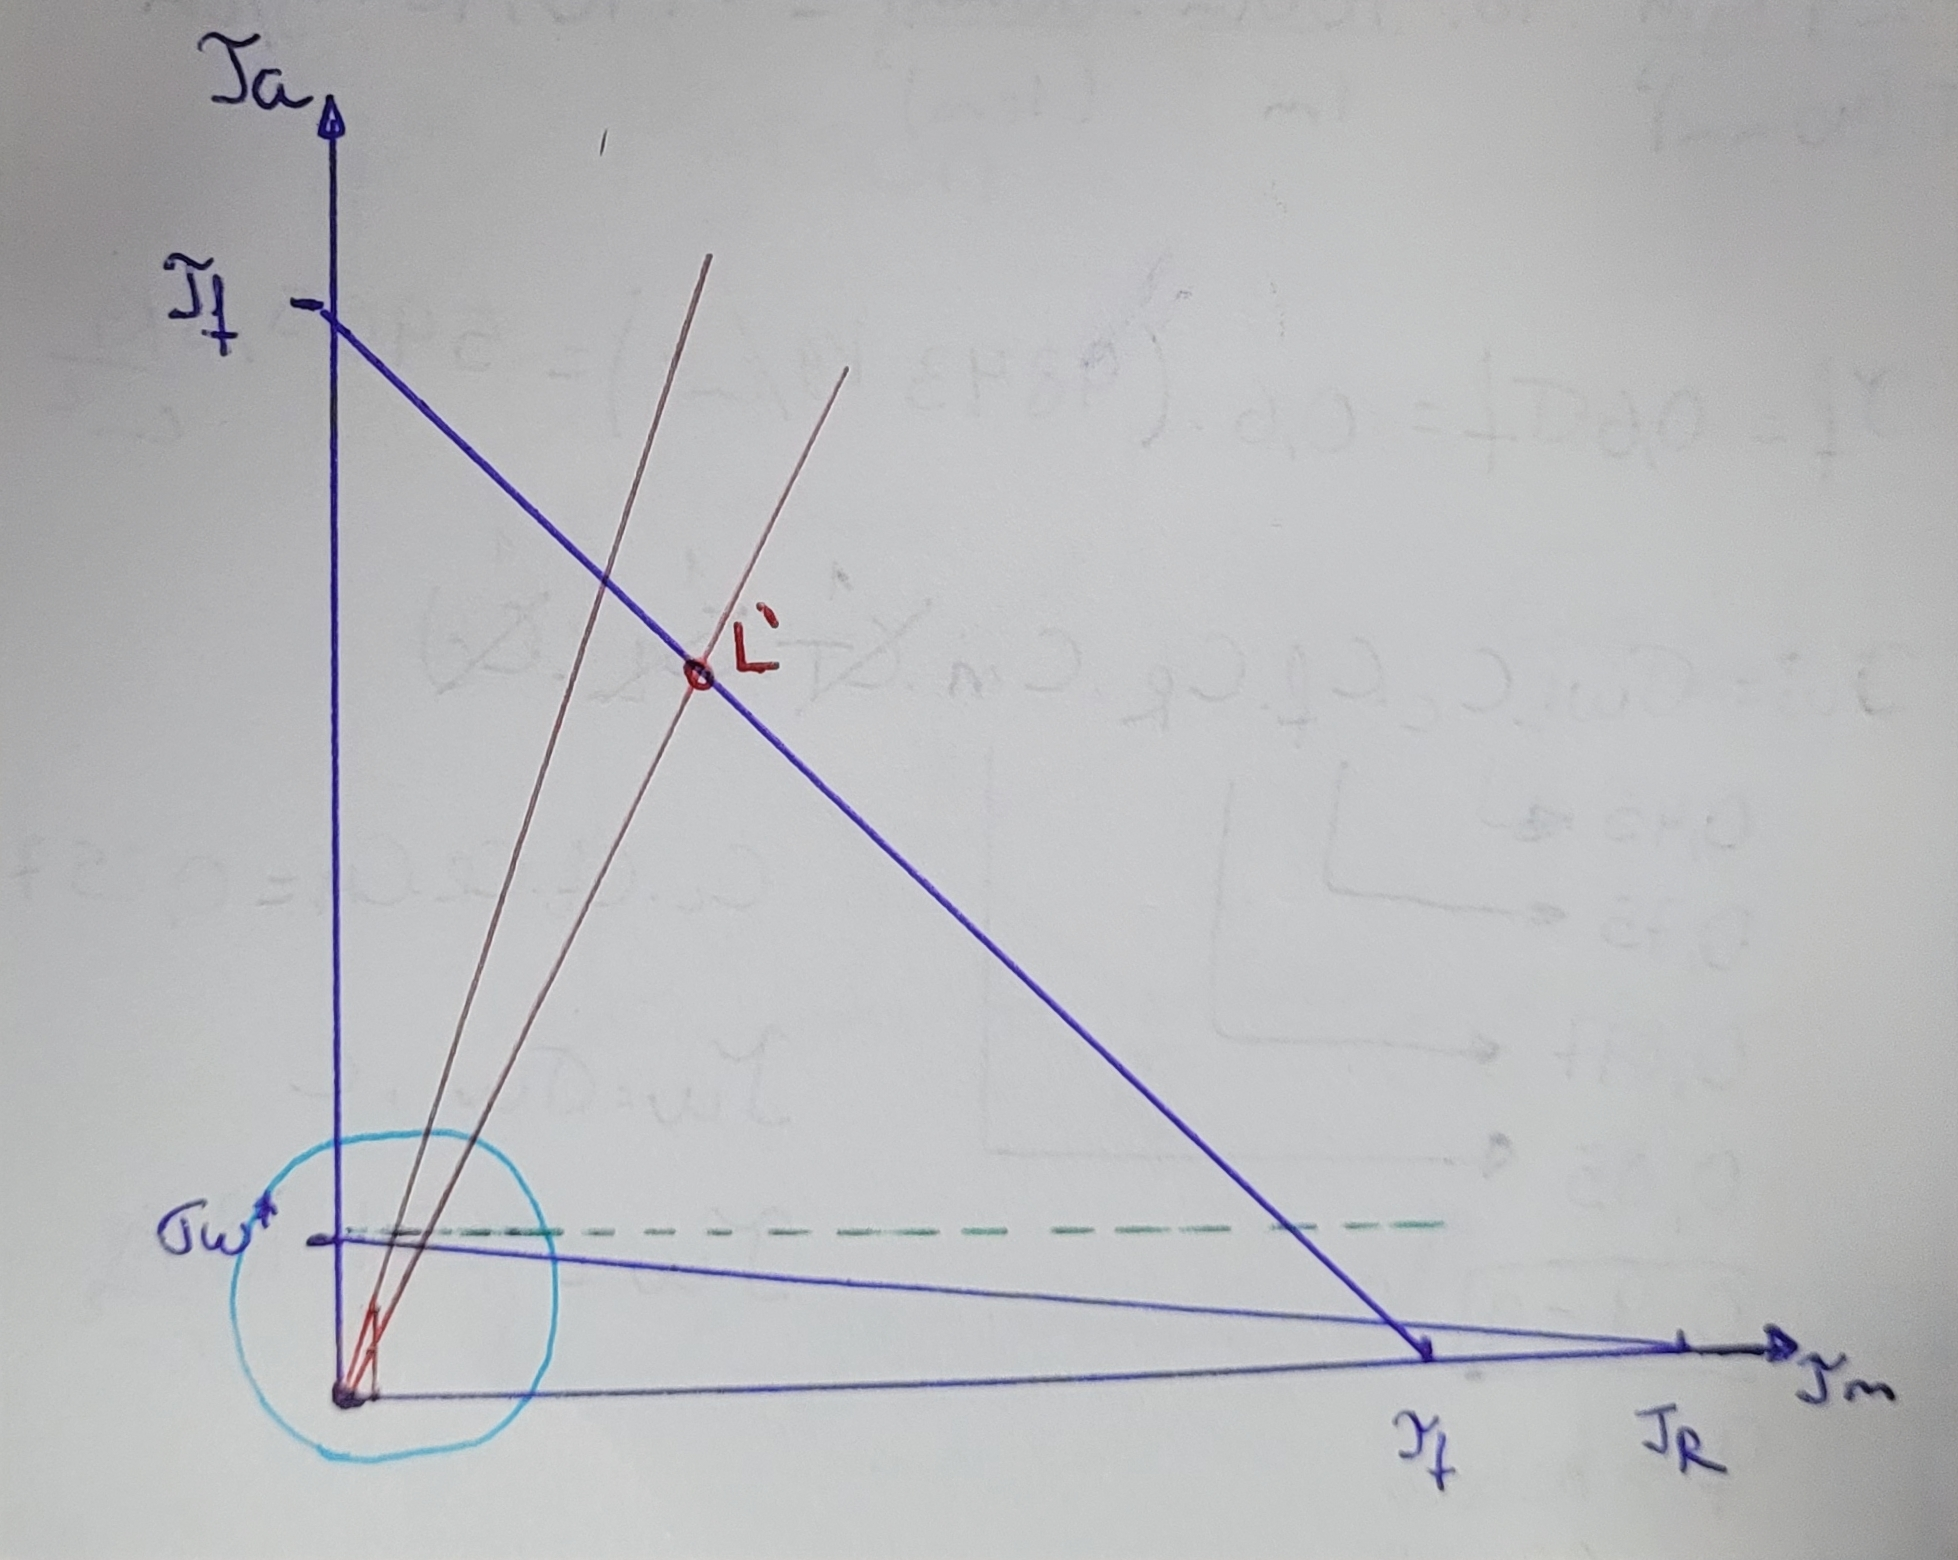
\includegraphics[width=0.8\textwidth]{goodman}\\
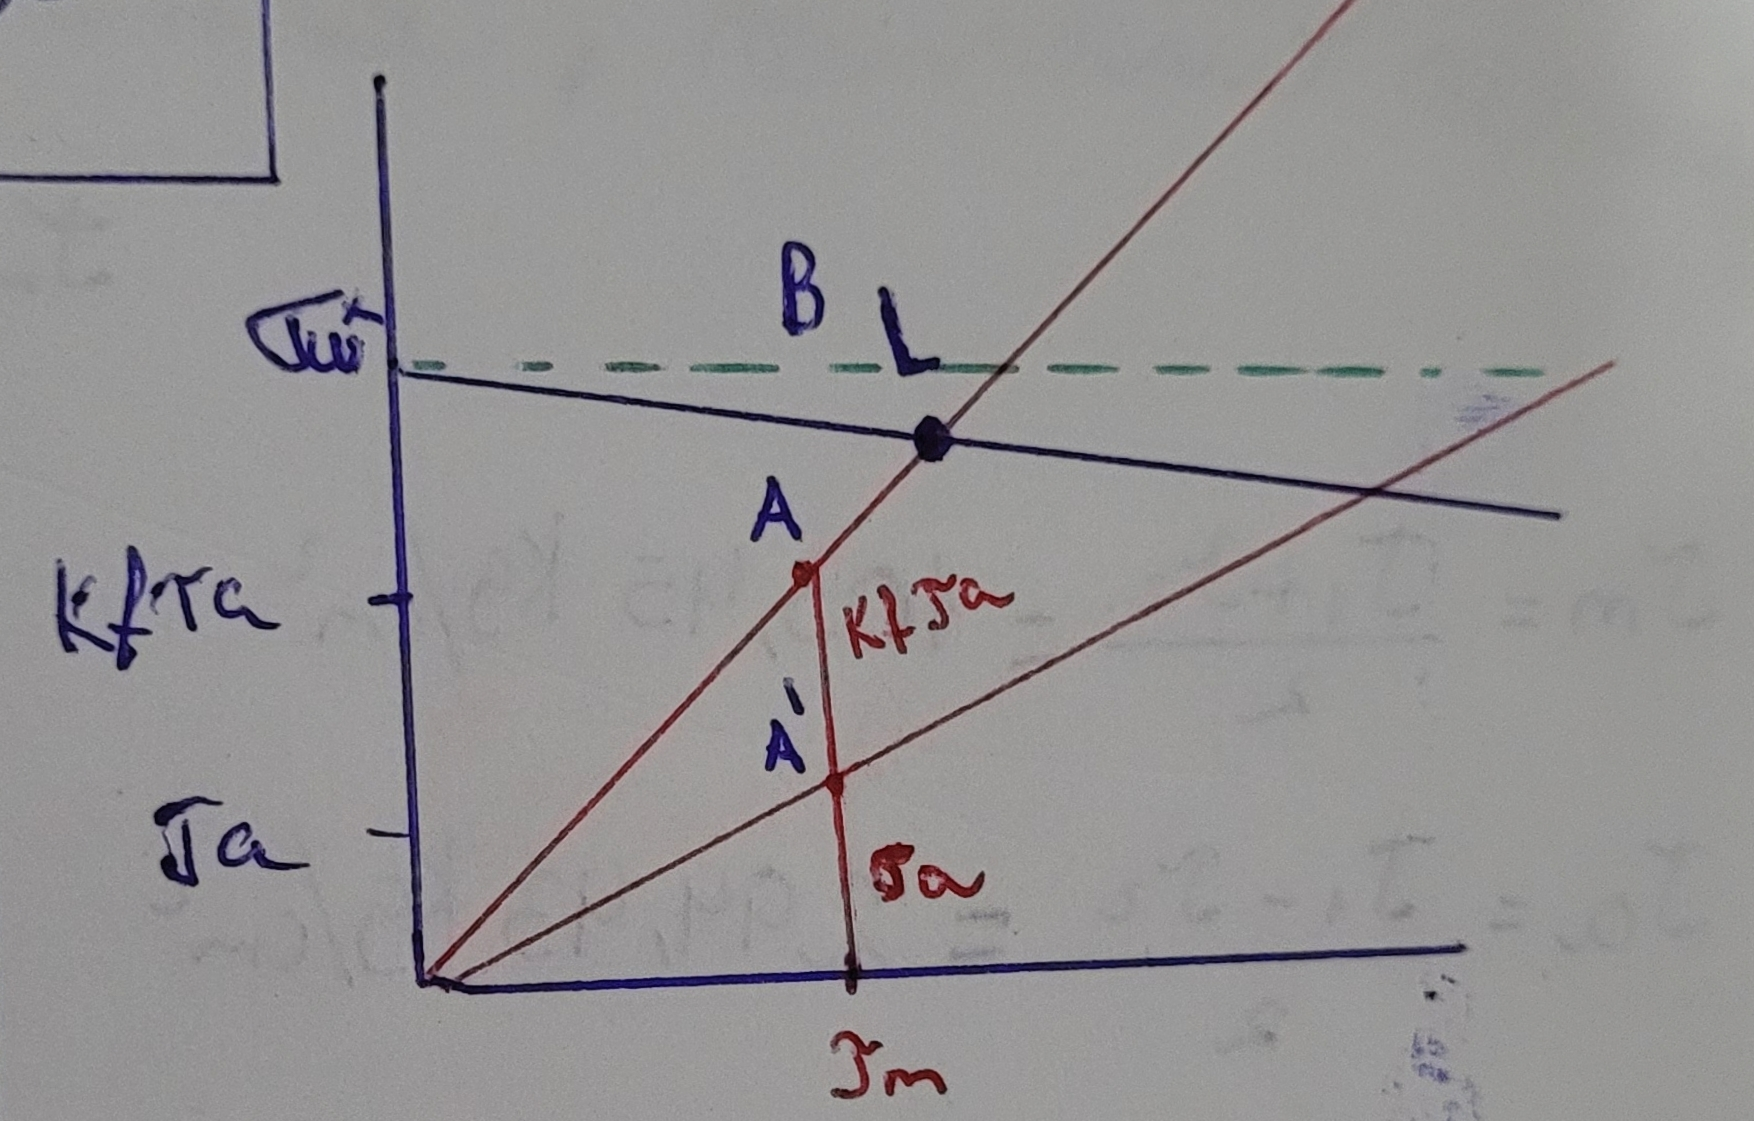
\includegraphics[width=0.8\textwidth]{goodman2}\\

\vspace*{0.2cm}
\begin{tabular}{l c r}	
	Soderberg&Cs&$\frac{OL}{OA}$\\[0.2cm]
	Elastico&Cs&$\frac{OL'}{OA'}$\\[0.2cm]
	Fatiga&Cs&$\frac{O'B}{O'A}$\\[0.2cm]
\end{tabular}
	\end{cajita}
	\newpage
%	\begin{cajita}
	% \justify
		\textbf{ENGRANAJES}\\
	\textbf{rectos: dimensionamiento}\\
			Carga transmitida $P_t$, la fuerza:\\
			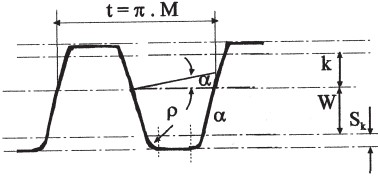
\includegraphics[height=0.2\textwidth]{engranaje-recto}\\
			\begin{tabular}{l l}
				Altura diente & $k + W$\\
							&$\rightarrow~De=Di+2h=Dp+2k$\\
				Altura de cabeza (k) & $k= M$ o $K=0.8M$\\
				Raíz (w) & $w=1.166M$\\
				Juego de cabeza& $S_k=W-k$\\
			\end{tabular}\vspace*{0.2cm}


			 $P_t=71620\dfrac{N}{n~\frac{Dp_1}{2}} \left[\dfrac{cv}{\frac{v}{min}~cm}\right]~\left[kg\right]$\\ \vspace*{0.2cm}
			Relación de transmisión : $i=\frac{\omega_2}{\omega_1}=\frac{z_1}{z_2}=\frac{Dp_1}{Dp_2}$\\ \vspace*{0.2cm}
			Paso del dentado: $z~t=\pi~Dp \rightarrow Dp=\frac{t}{\pi~z}=\frac{M}{\pi}$\\\vspace*{0.2cm}
			Módulo del dentado:\\\vspace*{0.2cm}
			\begin{centering}
				\begin{tabular}{l}
					Métrico/alemán\\
					$M(mm)=\dfrac{t(mm)}{\pi}=\dfrac{Dp(mm)}{z}$\\
					Diamteral pitch\\
					$P"(\frac{1}{pulg})=\dfrac{\pi}{t(")}=\dfrac{z}{Dp(")}$\\
				\end{tabular}
			\end{centering}\\\vspace*{0.2cm}
			Entre centro:\\
			$ec=\dfrac{dp_1+dp_2}{2}=\dfrac{M z_1+ M z_2}{2}=\frac{M}{2}(z_1+z_2)$\\


%	\end{cajita}

	\textbf{Ejes helicoidales}\\
	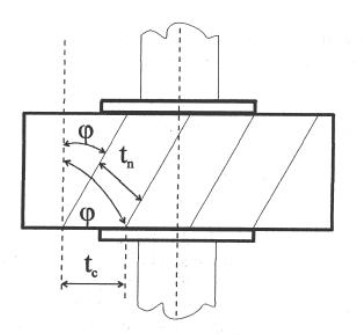
\includegraphics[width=0.3\textwidth]{engranaje-heli.jpg}\\
	\begin{tabular}{r l}
		$t_c$& paso circunferencial\\
		$t_n$& paso normal\\
	\end{tabular}\\
	\begin{tabular}{r l}
		$t_n\approx t_c Cos(\phi)$& $M_c=\dfrac{t_c}{\pi}$ \\
		\multicolumn{2}{c}{$M_n=\dfrac{t_n}{\pi}=M_c Cos(\phi)$}\\
	\end{tabular}\\
	
	$D_p=M_c z= \dfrac{M_n}{Cos(\psi)}z$\\
	$D_{ext}=D_p+2M_n =\dfrac{M_n}{Cos(\psi)}z+2M_n$\\
	$M_n=\dfrac{D_{ext}}{\frac{z}{Cos(\psi)}+2}$\\\vspace*{0.2cm}
	Entre centro:\\\vspace*{0.2cm}
	$ec=\dfrac{dp_1+dp_2}{2}=\dfrac{M_c z_1+ M z_2}{2}$\\
	$ec=\dfrac{M_n}{2 Cos{\psi}}(z_1+z_2)$\\
%	\begin{cajita}
	\vspace*{0.2cm}
		\textbf{Ejes concurrentes}\\


	\vspace*{0.2cm}
		\textbf{Ejes alabeados}\\
		\begin{tabular}{r l}
			$t_c$& paso circunferencial\\
			$t_n$& paso normal\\
			$m$& número filetes del piñon\\
			$i$&		Relacion transmición\\
		\end{tabular}\\

		\begin{tabular}{l l} $i$&$=\dfrac{\omega_2}{\omega_1}=\dfrac{R_1 ~ cos(\psi_1)}{R_2 ~ cos(\psi_2)}=\frac{m}{z_2}$\\
		$t_n$&$=\dfrac{2\pi R_1 cos(\psi_1)}{Z_1}$\\
		\end{tabular}\\
		En la elección de los ángulos se plantea:\\
		$\left\{\begin{array}{l}
			\phi=\psi_1+\psi_2\\
			i=\dfrac{R_1 ~ cos(\psi_1)}{R_2 ~ cos(\psi_2)}=\frac{m}{z_2}
		\end{array} \right.$
		
		
		
		
%	\end{cajita}
	\end{multicols}
\end{document}